\documentclass[tikz,border=6pt]{standalone}
\usetikzlibrary{arrows.meta}
\definecolor{red}{HTML}{A50F2D}\definecolor{ink}{HTML}{141414}\definecolor{gry}{HTML}{5F5F5F}\definecolor{blu}{HTML}{1F5F99}\definecolor{gn}{HTML}{1B7F5F}
% chain: \chain{y}{s1,...}{arc list handled below}
\newcommand{\bead}[3]{\fill[#3] (#1,#2) circle (0.12);}
\begin{document}
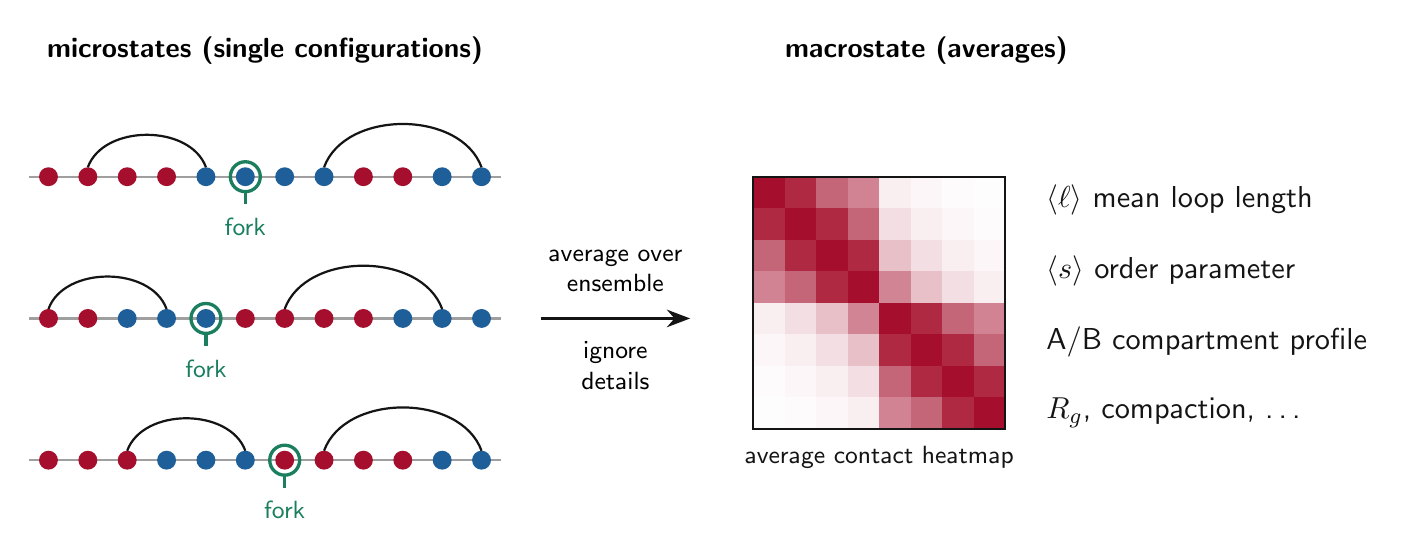
\begin{tikzpicture}[font=\sffamily\fontsize{11}{13}\selectfont,>=Stealth]
\node[font=\sffamily\bfseries] at (3.0,6.3) {microstates (single configurations)};
% three microstates
\foreach \k/\y in {1/4.7,2/2.9,3/1.1}{
  \draw[gry!60,thick] (0,\y)--(6,\y);
  \foreach \i in {0,...,11}{\fill[gry] ({0.5*\i+0.25},\y) circle (0.001);}
}
% microstate 1
\foreach \i/\c in {0/red,1/red,2/red,3/red,4/blu,5/blu,6/blu,7/blu,8/red,9/red,10/blu,11/blu}{\fill[\c] ({0.5*\i+0.25},4.7) circle (0.12);}
\draw[ink,thick] ({0.5*1+0.25},4.82) to[bend left=70] ({0.5*4+0.25},4.82);
\draw[ink,thick] ({0.5*7+0.25},4.82) to[bend left=70] ({0.5*11+0.25},4.82);
\draw[gn,very thick] (2.75,4.7) circle (0.19);\draw[gn,very thick] (2.75,4.51)--(2.75,4.35);\node[gn,font=\sffamily\small,anchor=north] at (2.75,4.3) {fork};
% microstate 2
\foreach \i/\c in {0/red,1/red,2/blu,3/blu,4/blu,5/red,6/red,7/red,8/red,9/blu,10/blu,11/blu}{\fill[\c] ({0.5*\i+0.25},2.9) circle (0.12);}
\draw[ink,thick] ({0.5*0+0.25},3.02) to[bend left=70] ({0.5*3+0.25},3.02);
\draw[ink,thick] ({0.5*6+0.25},3.02) to[bend left=70] ({0.5*10+0.25},3.02);
\draw[gn,very thick] (2.25,2.9) circle (0.19);\draw[gn,very thick] (2.25,2.71)--(2.25,2.55);\node[gn,font=\sffamily\small,anchor=north] at (2.25,2.5) {fork};
% microstate 3
\foreach \i/\c in {0/red,1/red,2/red,3/blu,4/blu,5/blu,6/red,7/red,8/red,9/red,10/blu,11/blu}{\fill[\c] ({0.5*\i+0.25},1.1) circle (0.12);}
\draw[ink,thick] ({0.5*2+0.25},1.22) to[bend left=70] ({0.5*5+0.25},1.22);
\draw[ink,thick] ({0.5*7+0.25},1.22) to[bend left=70] ({0.5*11+0.25},1.22);
\draw[gn,very thick] (3.25,1.1) circle (0.19);\draw[gn,very thick] (3.25,0.91)--(3.25,0.75);\node[gn,font=\sffamily\small,anchor=north] at (3.25,0.7) {fork};
% arrow
\draw[->,ink,very thick] (6.5,2.9)--(8.4,2.9);
\node[align=center,font=\sffamily\small] at (7.45,3.5) {average over\\ensemble};
\node[align=center,font=\sffamily\small] at (7.45,2.3) {ignore\\details};
% macrostate
\node[font=\sffamily\bfseries] at (11.4,6.3) {macrostate (averages)};
% heatmap
\foreach \i in {0,...,7}{\foreach \j in {0,...,7}{
  \pgfmathsetmacro{\v}{max(0, 100*exp(-abs(\i-\j)/1.5) + 38*(((\i<4)&&(\j<4))||((\i>=4)&&(\j>=4))) )}
  \pgfmathsetmacro{\vv}{min(\v,100)}
  \fill[red!\vv!white] ({9.2+0.4*\i},{3.4+0.4*(7-\j)-1.9}) rectangle ++(0.4,0.4);}}
\draw[ink,thick] (9.2,1.5) rectangle (12.4,4.7);
\node[ink,font=\sffamily\small,anchor=north] at (10.8,1.4) {average contact heatmap};
% numbers
\node[ink,anchor=west,align=left] at (12.8,4.4) {$\langle \ell \rangle$ mean loop length};
\node[ink,anchor=west,align=left] at (12.8,3.5) {$\langle s\rangle$ order parameter};
\node[ink,anchor=west,align=left] at (12.8,2.6) {A/B compartment profile};
\node[ink,anchor=west,align=left] at (12.8,1.7) {$R_g$, compaction, \dots};
\end{tikzpicture}
\end{document}
